% upLaTeX, dvipdfmxによるBeamerポスター
\documentclass[dvipdfmx, final, t]{beamer}
\usetheme{FJNKT98}

\usepackage{tabularx}   % 表を書く為

\usepackage{amsmath}    % 数式を書く為
\usepackage{bm}         % ボールド

\usepackage{url}      % URLを書くため
\usepackage{siunitx}  % SI単位を書くため

% 縦書き,A0サイズ
\usepackage[orientation=portrait,size=a0,scale=1.4]{beamerposter}

\title{ポスターのサンプル}
\author{fjnkt98}
\institute{NITIC}
\date{\today}

\begin{document}
\begin{frame}
  \begin{columns}[t]
    \begin{column}{.45\linewidth}
      \begin{block}{はじめに}
        \LaTeX でポスター!
      \end{block}

      \begin{block}{ほげほげ}
        \begin{itemize}
          \item 箇条書き
          \item いろいろ
          \begin{itemize}
            \item サブアイテム
            \begin{itemize}
              \item サブサブアイテム
            \end{itemize}
          \end{itemize}
        \end{itemize}

        \begin{enumerate}
          \item 数字付き箇条書き
          \item も出来るよ
        \end{enumerate}
      \end{block}

      \begin{block}{数式の例}
        \begin{equation*}
        {}^0\!T_{1}=\begin{pmatrix} C_{1} & -S_{1} & 0 & 0 \\ S_{1} & C_1 & 0 & 0 \\ 0 & 0 & 1 & 0 \\ 0 & 0 & 0 & 1 \end{pmatrix}
        \end{equation*}
      \end{block}

      \begin{block}{表の例}
        \begin{table}[h]
          \begin{tabular}{llll}
            \noalign{\hrule height 1pt}
            物質  & 記号 & 分子量 & 密度 \\
            \hline
            水   & H$_2$0 & 18.02 & 1.00 \\
            アルミ & Al & 26.98 & 2.70 \\
            銅   & Cu & 63.55 & 8.94 \\
            %\noalign{\hrule height 1pt}
          \end{tabular}
        \end{table}
      \end{block}
    \end{column}

    \begin{column}{.45\linewidth}
      \begin{block}{もげ}
        \structure{強調表現!}

        \alert{これも強調表現!}

        \begin{figure}[h]   % h: この場所に t: ページのトップに b: ページのボトムに p: 新しいページを作って画像を貼る
          \centering              % 中央揃え
          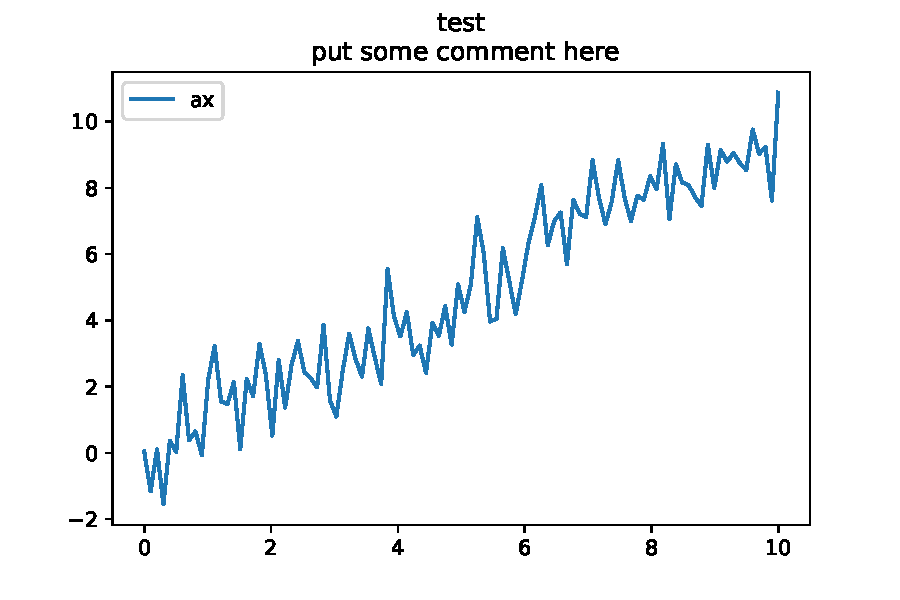
\includegraphics[width=180truemm,clip]{images/graph_sample.pdf}
          \caption{Sample Picture}% 図のタイトル(英語)
          \label{fig:sample}      % 参照用ラベル
      \end{figure}
      \end{block}

      \begin{alertblock}{アラート}
        アラートブロック
      \end{alertblock}
    \end{column}
  \end{columns}
\end{frame}
\end{document}